%  article.tex (Version 3.3, released 19 January 2008)
%  Article to demonstrate format for SPIE Proceedings
%  Special instructions are included in this file after the
%  symbol %>>>>
%  Numerous commands are commented out, but included to show how
%  to effect various options, e.g., to print page numbers, etc.
%  This LaTeX source file is composed for LaTeX2e.

%  The following commands have been added in the SPIE class 
%  file (spie.cls) and will not be understood in other classes:
%  \supit{}, \authorinfo{}, \skiplinehalf, \keywords{}
%  The bibliography style file is called spiebib.bst, 
%  which replaces the standard style unstr.bst.  

\documentclass[A4]{spie}  %>>> use for US letter paper
%%\documentclass[a4paper]{spie}  %>>> use this instead for A4 paper
%%\documentclass[nocompress]{spie}  %>>> to avoid compression of citations
%% \addtolength{\voffset}{9mm}   %>>> moves text field down
%% \renewcommand{\baselinestretch}{1.65}   %>>> 1.65 for double spacing, 1.25 for 1.5 spacing 
%  The following command loads a graphics package to include images 
%  in the document. It may be necessary to specify a DVI driver option,
%  e.g., [dvips], but that may be inappropriate for some LaTeX 
%  installations. 
\usepackage[]{graphicx}

\title{Absolute calibration of gravitational wave detector using gravity field and photon pressure} 

%>>>> The author is responsible for formatting the 
%  author list and their institutions.  Use  \skiplinehalf 
%  to separate author list from addresses and between each address.
%  The correspondence between each author and his/her address
%  can be indicated with a superscript in italics, 
%  which is easily obtained with \supit{}.

\author{Yuki Inoue\supit{a,b}, Sadakazu Haino\supit{a}, Nobuyuki Kanda\supit{c}, Yujiro Ogawa\supit{b.d}, Toshikazu Suzuki\supit{b,e}, Takayuki Tomaru\supit{b,d,e}, Takahiro Yamamoto\supit{f}, Takaaki Yokozawa\supit{f}
\skiplinehalf
\supit{a}Institute of Physics, Academia Sinica, Nankang, Taipei 11529, Taiwan; \\
\supit{b}High Energy Accelerator Research Organization, Tsukuba, Ibaraki, 305-0801, Japan;\\
\supit{c}Department of Physics, Osaka City University, Sumiyoshi, Osaka 558-8585, Japan;\\
\supit{d}SOKENDAI (The Graduate University for Advanced Studies), Hayama, Miura District, Kanagawa 240-0115, Japan;\\
\supit{e}Institute for Cosmic Ray Research, University of Tokyo, Kashiwa, Chiba, 277-8582, Japan;\\
\supit{f}KAGRA Observatory, Institute for Cosmic Ray Research, University of Tokyo, Hida, Gifu 506-1205, Japan;\\
}

%>>>> Further information about the authors, other than their 
%  institution and addresses, should be included as a footnote, 
%  which is facilitated by the \authorinfo{} command.

\authorinfo{Yuki Inoue: iyuki@post.kek.jp}
%%>>>> when using amstex, you need to use @@ instead of @
 

%%%%%%%%%%%%%%%%%%%%%%%%%%%%%%%%%%%%%%%%%%%%%%%%%%%%%%%%%%%%% 
%>>>> uncomment following for page numbers
% \pagestyle{plain}    
%>>>> uncomment following to start page numbering at 301 
%\setcounter{page}{301} 
 
\begin{document} 
\maketitle 

%%%%%%%%%%%%%%%%%%%%%%%%%%%%%%%%%%%%%%%%%%%%%%%%%%%%%%%%%%%%% 
\begin{abstract}
Absolute calibration of the gravitational wave detectors is an essential to evaluate the various parameters of the gravitational wave sources. 
The photon calibrator is primary calibrator for calibrating the absolute displacement of the mirror by using the photon pressure. 
Current technological limit of the absolute calibration uncertainty is 3.5 \% corresponding to the uncertainty of the laser power standard of the standard metrology institutes from nine country.  In order to reduce the uncertainty of the photon calibrator, we propose a new method using the combination of photon calibrator and gravity field calibrator. The gravity field calibrator gives the modulation to mirror using the gravity gradient. In previous study, uncertainty of the distance between the test mass and gravity field calibrator is one of the serious systematic error of the absolute calibration. To cancel this uncertainty, we newly propose the method of quadrupole and hexapole mass distribution.  We also estimated the uncertainty of this method. The estimated precision of absolute calibration is 0.3\%, which is 10 times less than that of previous method.

\end{abstract}

%>>>> Include a list of keywords after the abstract 

\keywords{Gravitational Wave, KAGRA, LIGO, Virgo, Calibration}

%%%%%%%%%%%%%%%%%%%%%%%%%%%%%%%%%%%%%%%%%%%%%%%%%%%%%%%%%%%%%
\section{Introduction}

%Overview of GW observation
The discovery of the gravitational wave (GW) gave us the new probe for observing our universe~\cite{PhysRevLett.116.061102}. 
The typical strain sensitivity, $h$, of 2nd generation interferometric detectors (IFO), such as Advanced LIGO~\cite{0264-9381-32-7-074001}, Advanced Virgo~\cite{0264-9381-32-2-024001}, and KAGRA~\cite{0264-9381-29-12-124007, PhysRevD.88.043007}, are around $10^{-23}/\sqrt{Hz}$ at 100 Hz. 
% Added by SH 180412
By using the GW signals from compact binary coalescences, we can derive 
the parameters such as masses, spins, luminosity distance, orbital inclination 
and the sky location of the binary system from the detected waveforms. 
The precision of the derived parameters are potentially limited by the 
calibration accuracy. As the number of detected sources increases and we 
detect higher signal-to-noise ratio (SNR) events, the calibration uncertainty 
will become the dominant source of the errors to extract physics information. 
In particular, the uncertainty on the absolute GW signal amplitude directly 
propagates to the error on the estimation of the distance to the sources. 
The detection of GW signal from a Binary Neutron Star (BNS) system, 
GW170817~\cite{GW170817:2017aa} in both GW and Electro-Magnetic (EM) 
waves opened a new era of multi-messenger astronomy. These observations 
allow us to use GW170817 as a standard 
siren~\cite{Abbott:2017xzu,Schutz_1986,Holz_2005,Nissanke_2010} to 
determine the absolute luminosity distance to the source directly from the 
GW signal measurements. Assuming the event rate of 3000 Gpc$^{-3}$yr$^{-1}$ 
which is consistent with the bounds from GW170817 at 90\% 
confidence~\cite{GW170817:2017aa}, we expect to detect GW signals from about 
50 BNS standard sirens in the next few observing runs. 
They can constrain the Hubble constant ($H_0$) 
measurement to 2\% or less~\cite{Feeney:2018mkj}, and eventually resolve 
the 3-$\sigma$ tension of the $H_0$ measurement between Cephied-SN distance 
ladder~\cite{Riess_2016} and CMB data assuming a $\Lambda$CDM 
model.~\cite{2016-planck} The systematic errors on the calibration of 
the absolute GW signal amplitude must be suppressed at the sub-\% level to 
achieve the high precision $H_0$ measurement with the GW standard sirens.

% Commented out by SH 180412
%In order to estimate the parameters of gravitational waves, such as masses, spins, redshift and distance, understanding of the systematic and statistical noise sources are critical.
%In particular, the uncertainty of the absolute calibration directly propagate to the estimation error of the distance of the GW sources. The multi messenger observations of the binary neutron star, GW170817, open the new method to estimate the Hubble constant. The accuracy of estimation of the constant is proportional to the systematic uncertainties of source distance. 
% Commented out by SH 180412

%To understand the origin of heavier binary black hole, we need to obtain the precise mass and distance distribution. So, the improvement of absolute calibration is one of the important topic for the future gravitational wave astronomy.

%Calibration
An interferometer measures the change of distance difference along the two arms of interferometer. Then, the fluctuations in the degree of freedom of differential arm length (DARM) is suppressed by the DARM control loop. The reconstruction signal of DARM fluctuation at the observation frequency is excited by the gravitational waves. We can reconstruct the gravitational waveform with the calibrated error and control signals of this DARM loop. To calibrate the signals, the accurate modelings of the actuator and sensing function are essential. To understand the model, we need to measure the transfer function and monitor the time dependency of the transfer function using continuous sine curve (calibration lines). The residual of the time-dependent models corresponds to uncertainty of the detection.

%Pcal
To reduce the calibration systematic uncertainty, we need to inject well parameterized calibration line by photon calibrator (Pcal) or other calibration source for monitoring the time variation of the response of IFO. The first generation of the photon calibrator was developed by the Glasgow and GEO600~\cite{CLUBLEY200185,MOSSAVI20061}. They proposed the modulation method with photon pressure for understanding the response of interferometer. The second generation photon calibrator is developed by LIGO~\cite{doi:10.1063/1.4967303,0264-9381-27-8-084024,0264-9381-26-24-245011,0264-9381-32-2-024001}. LIGO and Virgo employ the second generation photon calibrator for the calibration of time-dependent response of IFO~\cite{0264-9381-32-2-024001}. The third generation photon calibrator is developed by KAGRA~\cite{KAGRA_Pcal}. KAGRA employ the 20~W laser and independent modulation system for injected beams. LIGO and KAGRA use a power sensor called to as the Gold standard, which is calibrated by the laser power standard of NIST in Boulder, CO~\cite{taylor:1994:GEEU}. However, it has a challenging issue of the absolute calibration due to the accuracy of the absolute laser power of laser standard between national metrology institute from nine countries. The 
systematic discrepancies between nine countries are as large as 3.5~\%~\cite{EUROMET}.

%KAGRA and Our approach
The dynamic gravity field calibrator (Gcal) is one of the candidates to be able to solve the uncertainty problem of absolute calibration. The technologies of the system are established and tested in Forward and Miller~\cite{doi:10.1063/1.1709366}, Weber~\cite{PhysRevLett.18.795,PhysRev.167.1145}, University of Tokyo~\cite{Hirakawa,1347-4065-19-3-L123,1347-4065-20-7-L498,PhysRevD.26.729,PhysRevD.32.342} and Rome university group~\cite{Astone1991}. Related techniques using gravity field calibrator for the calibration are discussed in Matone et al \cite{0264-9381-24-9-005}. It can modulate the test mass using gravity gradient with rotor. The amplitude of displacement of the mirror is determined by masses, distance, frequency, radius, and gravity constant. 
%Chap1 is XXXXX, … .

In this paper, we propose how we can achieve sub-percent uncertainty of the calibration. We focus on the combination method of the photon calibrator and gravity field calibrator.
In section~\ref{sec:Pcal}, we explain how to calibrate with photon calibrator. In chapter~\ref{sec:Gcal}, we show the principle of multipole moment gravity and modulation method.
In section \ref{sec:PGCAL}, we show how to calibrate the absolute displacement with Pcal and Gcal. In section~\ref{sec:EST}, we discuss the systematic error by changing parameters.

\section{Photon calibrator} \label{sec:Pcal}
Pcal relies on the photon radiation pressure from the power modulated laser beams reflecting on the test mass to apply periodic force via the recoil of photons~\cite{doi:10.1063/1.4967303}. 
advanced LIGO, advanced Virgo and KAGRA employ the photon calibrator for the calibration of the interferometer response~\cite{0264-9381-34-1-015002, KAGRA_Pcal,0264-9381-32-2-024001}. Each gravitational detectors placed the 1047~nm laser around the end test mass. The displacement of the test mass can be described as
\begin{equation}
 x = \frac{P \cos{\theta}}{2c} s(\omega)\left(1+\frac{M}{I}\vec{a} \cdot \vec{b} \right) , \label{pcal}
\end{equation}
where $P$ is absolute laser power, $\theta$ is incident angle of the Pcal laser, $M$ is mass of test mass, $\omega$ is angular frequency of the laser power modulation, $\vec{a}$ and $\vec{b}$ are position vector of Pcal laser beams. The schematic view is shown in Fig.~\ref{fig:Pcal}. $I=Mh^2/12+Mr^2/4$ is the moment of inertia, where $h$ and  $r$ are thickness and radius of test mass. $s(\omega)$ is transfer function between force and displacements. We can regard the $s(\omega)$ as $1/(M \omega^2)$ above 20 Hz. 

The laser power is stabilized less than design sensitivity. The schematic view of the photon calibrator is shown in Fig.~\ref{fig:Pcal}. The stabilized laser is mounted on the transmitter module. The power is monitored by the response of the photo detectors at the transmitter module, $V_{\mathrm{TxPD}}$, and receiver module, $V_{\mathrm{RxPD}}$.  
The largest relative uncertainty of photon calibrator is that of laser power.
LIGO and KAGRA use the working standard to cross-calibrate the relative response of each interferometer. The relative uncertainty of  each  calibrator is 0.51 \%~\cite{doi:10.1063/1.4967303}. 
The second largest relative uncertainty is an optical efficiency of the optical path. We calibrate the injected power from the outside of the vacuum chamber. Therefore, we need to consider the optical efficiency due to the transmittance of the vacuum window and reflectance of the mirrors. The measured uncertainty of optical efficiency in LIGO is 0.37 \%. 
For the absolute calibration, the detector, so called ``Gold standard", is calibrated with the NIST laser power standard. After that, The responses of ``Working standard" of Hanford, Livingston and KAGRA are calibrated by the "Gold standard" in LIGO Hanford observatory. 
However, the result of comparison between accuracies of the absolute laser powers of each institutes has 3.5~\% uncertainty. It implies that the serious systematic error for distance estimation because the uncertainty of the absolute calibration propagate to the distance of the GW source.

\begin{figure}
\begin{center}
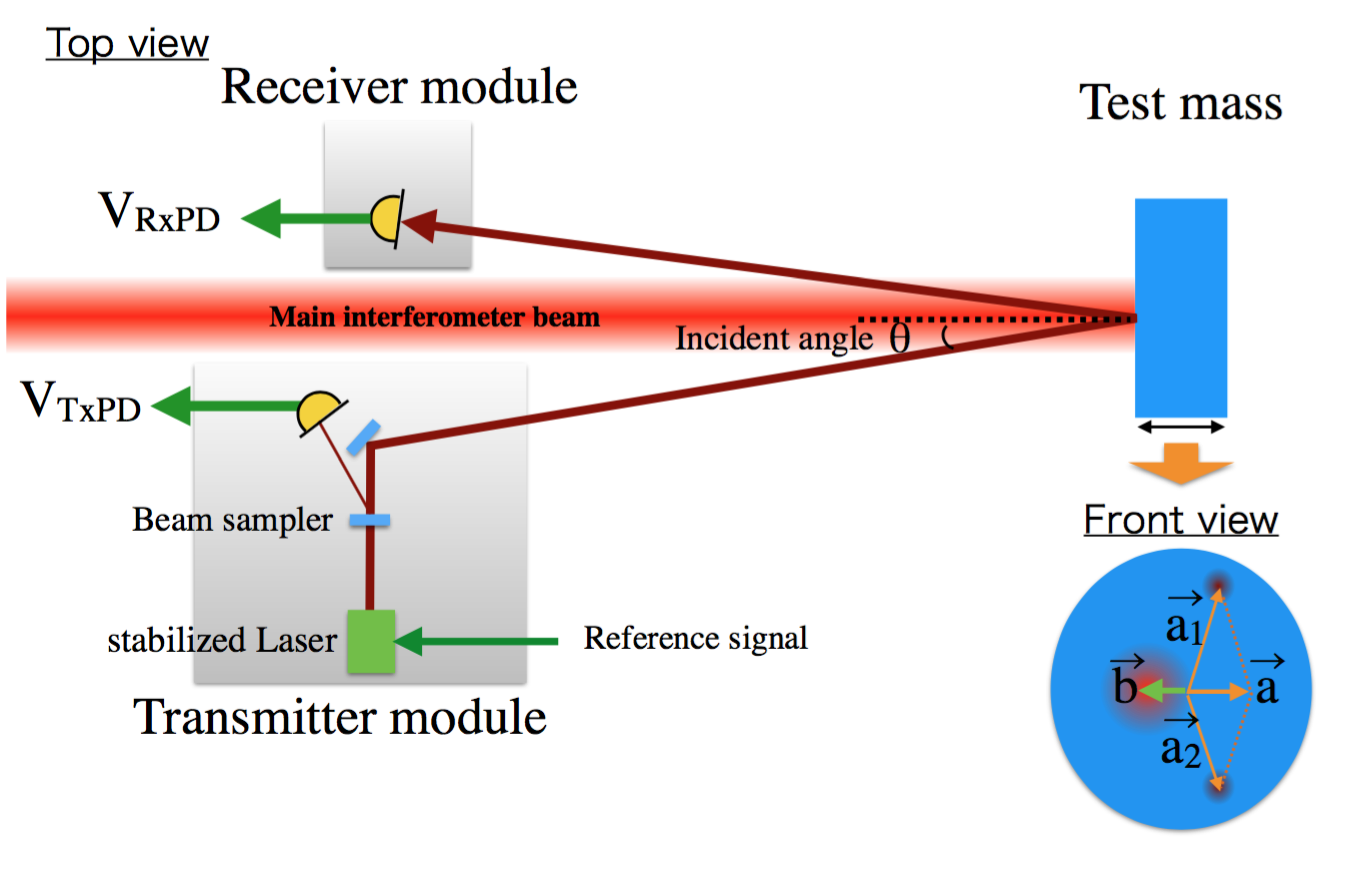
\includegraphics[width=12cm]{Pcal.eps}
\caption{Schematic view of photon calibrator. We place the stabilized laser on the transmitter module. The injected signal at the test masses is monitored by using the response of photo detector power between the transmitter module, $V_{TxPD}$ and  receiver module, $V_{RxPD}$.  The geometrical factor is characterized by the position vectors of photon calibrator beams, $\vec{a}=\vec{a_1}+\vec{a_2}$, and the main beam, $\vec{b}$.}
\label{fig:Pcal}
\end{center}
\end{figure}

\begin{table}
\begin{center}
\caption{Specification summary of LIGO, Virgo and KAGRA photon calibrator\label{pcal}}
\footnotesize
\begin{tabular}{cccc}
\hline
& KAGRA& advanced LIGO& advanced Virgo \\
\hline
Mirror material & Sapphire & Silica & Silica \\
 Mirror mass & 23 kg & 40 kg & 40 kg \\
  Mirror diameter & 220 mm & 340 mm & 350 mm \\
    Mirror thickness & 150 mm & 200 mm & 200 mm \\
 Distance of Pcal from ETM & 36 m & 8 m & 1.5 m \\
  Pcal laser power & 20 W & 2W & 3 W \\
  Pcal laser frequency & 1047 nm & 1047 nm &1047 nm\\
  Incident angle& 0.72 deg & 8.75 deg &30 deg \\
  \hline
\end{tabular}
\end{center}
\end{table}

\section{Gravity field calibrator} \label{sec:Gcal}
To solve the uncertainty problem of the absolute calibration, we propose the method of gravity field calibrator. The gravity field calibrator generate the dinamic gravity field at the end of test mass by rotating the multipole masses. The rotor placed in the vacuum chamber for isolating the acoustic noise. To monitor the frequency, we mount the 10-bit encoder. We read the response of encoder using 16 bit ADC system.
We calculated the displacement by changing dynamic gravity field of multipole moment with N peaces of masses.
We assumed the suspended test mass for the interferometer and disk with multipole masses as shown in Fig ~\ref{fig:dim}.
We put the masses, $m$, at the positions of the radius, $r$. The distance between the center of mass of mirror and disk is assumed $d$.
We rotate the disk at the angular frequency of $\omega_{\mathrm{rot}}=2\pi f_{\mathrm{rot}}$.

\begin{figure}
\begin{center}
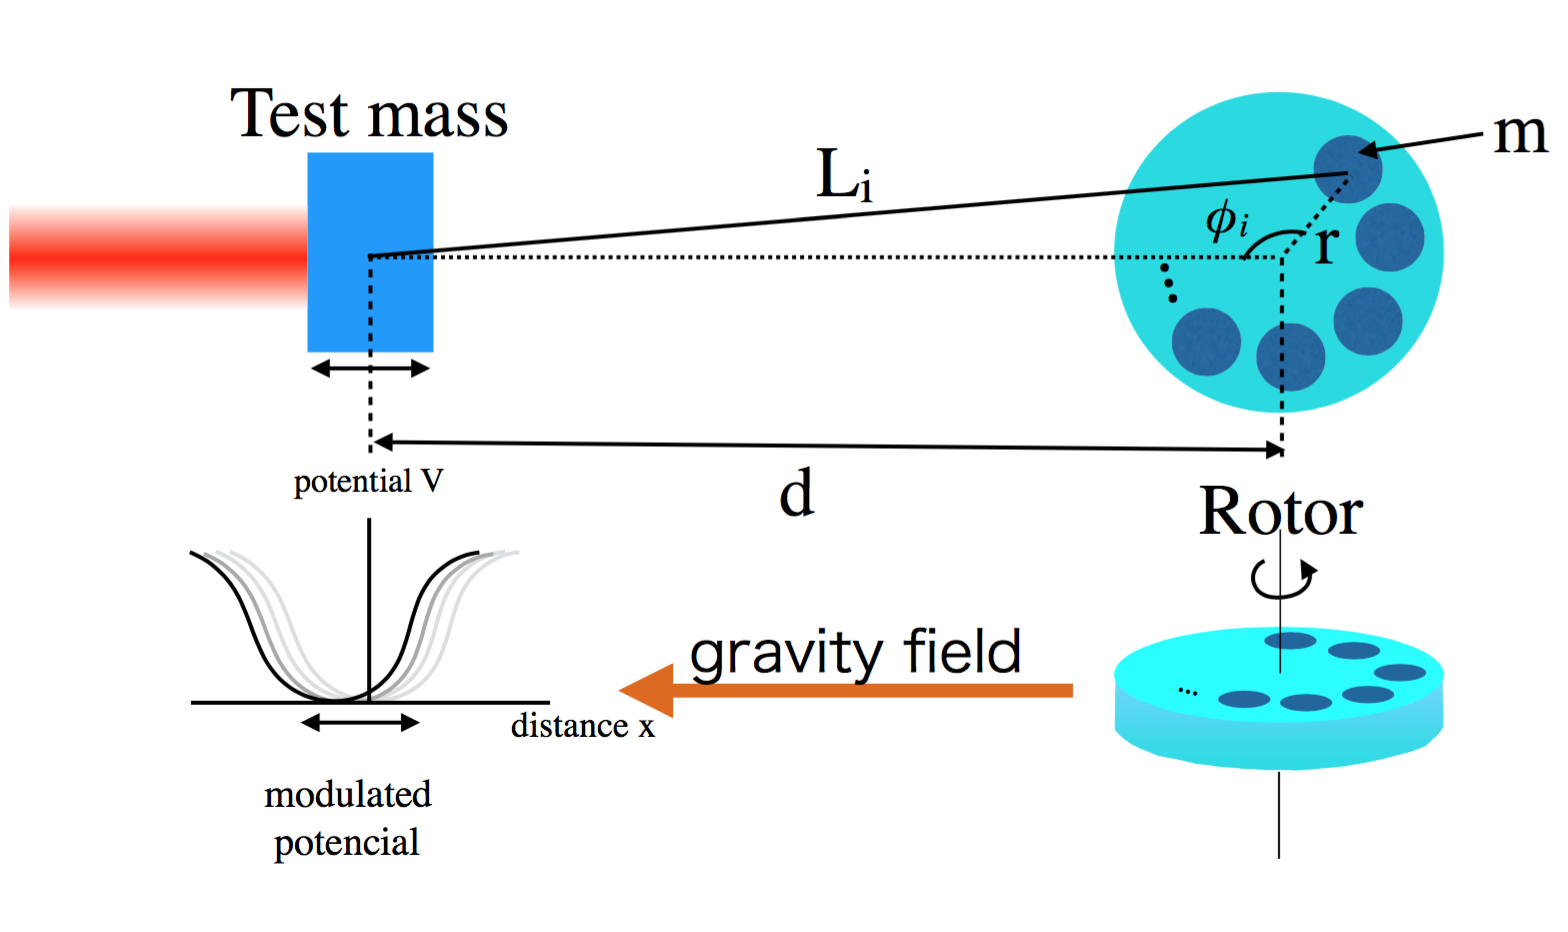
\includegraphics[width=12cm]{dim.eps}
\caption{Schematic view of gravity field calibrator. We placed the rotor at  the same hight and the distance of $d$ away from test masses. Multipole mass generate the gravitational potential at the test mass position.}
\label{fig:dim}
\end{center}
\end{figure}
First we calculate the distance with N pieces of masses which are separated by radius of r from the center of the rotor mass and arranged at equal intervals, respectively.
Distance between i-th mass and center of test mass is written as
\begin{equation}
L_i=d \sqrt{1+\left( \frac{r}{d} \right)^2 -2\left( \frac{r}{d} \right) \cos{\phi_i} },
\end{equation}
where the angle of i-th mass is assumed as $\phi_i=\omega_{\mathrm{rot}} t + 2\pi i/N$.
The gravity potential at the center of test mass can be described as
\begin{eqnarray}
V &=& \Sigma^N_{i=0} V_i \\
&=& -GMm \Sigma^N_{i=0}L_i^{-1}\\
&=&-\frac{GMm}{d} \Sigma^N_{i=0} \Sigma^{\infty}_{n=0} \left( \frac{r}{d} \right)^n P_n\left(\cos{\left(\omega_{\mathrm{rot}} t +\frac{2 \pi i}{N}\right)}\right),
\end{eqnarray}
where $P_n$ is Legendre polynomial, and $V_i$ is potential of a mass. The equation of motion of test mass is 
\begin{equation}
Ma=\left| \frac{\partial V}{\partial{d}} \right| =\frac{GMm}{d^2}\Sigma^N_{i=0} \Sigma^{\infty}_{n=0}(n+1) \left( \frac{r}{d} \right)^n P_n\left(\cos{\left(\omega_{\mathrm{rot}} t +\frac{2 \pi i}{N}\right)}\right),
\end{equation}
where $a$ is acceleration of test mass. 

We place the quadrupole and hexapole masses in the same rotor as shown in Fig.~\ref{fig:hex}. We put the hole between each mass. The hole can increase the gravity gradient twice effectively. Therefore, we can describe the equation of motion as 
\begin{equation}
Ma=\left| \frac{\partial V}{\partial{d}} \right| =\frac{2GMm}{d^2}\Sigma^N_{i=0} \Sigma^{\infty}_{n=0}(n+1) \left( \frac{r}{d} \right)^n P_n\left(\cos{\left(\omega_{\mathrm{rot}} t +\frac{2 \pi i}{N}\right)}\right). \label{eq:EOM}
\end{equation}
We will calculate the displacement of quadrupole and hexapole in the section ~\ref{Quad}  and ~\ref{Hexa}.

\begin{figure}
\begin{center}
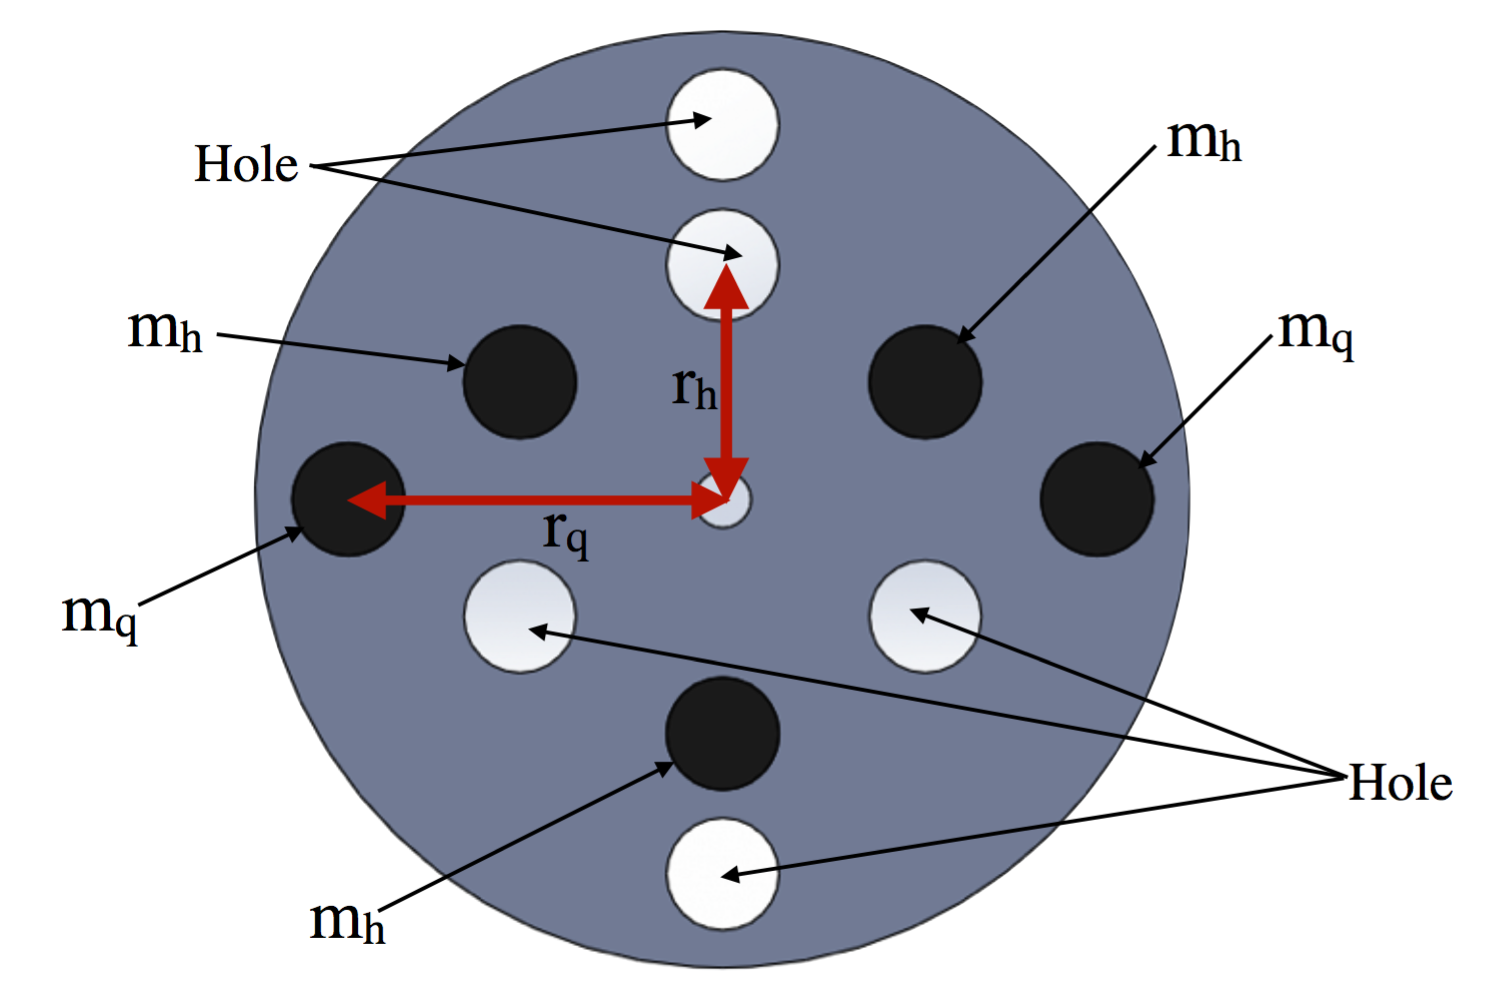
\includegraphics[width=12cm]{Hexapole.eps}
\caption{Configuration of the rotor with quadrupole and haxapole mass distribution. $m_{\mathrm{q}}$ and $m_{\mathrm{h}}$ are mass of quadrupole and hexapole. $r_{\mathrm{q}}$ and $r_{\mathrm{h}}$ are radius of quadrupole and hexapole.}
\label{fig:hex}
\end{center}
\end{figure}

\subsection{Displacement of test mass (Quadrupole)} \label{Quad}
We calculate the displacement of the quadrupole mass distribution corresponding to $N=2$.
The masses and radiuses of quadrupole are assumed as $m_{\mathrm{q}}$ and $r_{\mathrm{q}}$. 
The equation of motion of test mass is described as
\begin{equation}
Ma=\frac{2GMm_{\mathrm{q}}}{d^2}\Sigma^{\infty}_{n=0}(n+1) \left( \frac{r_{\mathrm{q}}}{d} \right)^n \left( P_n\left(\cos{\left(\omega_{\mathrm{rot}} t \right)}\right) + P_n\left(\cos{\left(\omega_{\mathrm{rot}} t +\pi \right)}\right) \right).
\end{equation} 
If we assume $r \ll d$, the displacement of the time-dependent lower harmonics can be written by 
\begin{equation}
x=\Sigma_{k=1}^{\infty}x_{k\mathrm{f}}\cos(k\omega_{\mathrm{rot}} t)\sim x_{\mathrm{2f}}\cos(2\omega_{\mathrm{rot}} t)=x_{\mathrm{2f}}\cos{\omega t},
\end{equation}
where $k$ is the number of the harmonics. 
The amplitude of 2-f rotation is described as
\begin{equation}
x_{2\mathrm{f}}=9\frac{GMm_{\mathrm{q}}r_{\mathrm{q}}^2}{d^4}s(\omega). \label{2f}
\end{equation}

\subsection{Displacement of test mass (Haxapole)} \label{Hexa}
We also calculate the displacement of the hexapole mass distribution, which corresponds to $N=3$.
The masses and radiuses of hexapole are assumed as $m_{\mathrm{h}}$ and $r_{\mathrm{h}}$. 
The equation of motion of test mass is described as
\begin{eqnarray}
Ma &=& \frac{2GMm_{\mathrm{h}}}{d^2}\Sigma^{\infty}_{n=0}(n+1) \left( \frac{r_{\mathrm{h}}}{d} \right)^n \nonumber \\ 
&&\times \left( P_n\left(\cos{\left(\omega_{\mathrm{rot}} t \right)}\right) + P_n\left(\cos{\left(\omega_{\mathrm{rot}} t+\frac{2\pi}{3} \right)} \right) + P_n\left(\cos{\left(\omega_{\mathrm{rot}} t \frac{4\pi}{3} \right) }\right) \right).
\end{eqnarray} 
If we assume $r \ll d$, the displacement of the time-dependent lower harmonics can be written by 
\begin{equation}
x=\Sigma_{k=1}^{\infty}x_{k\mathrm{f}}\cos(k\omega_{\mathrm{rot}} t)\sim  x_{3\mathrm{f}}\cos(3\omega_{\mathrm{rot}} t)=x_{\mathrm{3f}}\cos{\omega t},
\end{equation}
where amplitude of 3-f is described as
\begin{equation}
 x_{3\mathrm{f}}=15\frac{GMm_{\mathrm{h}}r_{\mathrm{h}}^3}{d^5}s(\omega). \label{3f}
\end{equation}

\section{Absolute power calibration by using Gcal and Pcal} \label{sec:PGCAL}
In this section, we discuss about absolute laser power calibration using interferometer. 
Figure~\ref{fig:IFO} shows the configuration of the calibration by using the combination of photon calibrator and gravity field calibrator.
First, we modulate the mirror position using gravity field calibrator. We can measure the signal of $x_{\mathrm{2f}}$ and $x_{\mathrm{3f}}$ in the response of interferometer. Second, we send the interferometer signal to the excitation port of photon calibrator as a reference signal port of feedback control as shown in Fig.~\ref{fig:IFO}. The photon calibrator cancel the displacement by gravity field calibrator. Third, we measure the response of the detector of transmitter module and receiver module, whose units are volt. The output signal of transmitter module, $V_{\mathrm{TxPD}}$ and receiver module, $V_{\mathrm{RxPD}}$ should be corresponding to displacement from gravity field. By using Eq~(\ref{pcal}),(\ref{2f}), and (\ref{3f}), the modulated powers are
\begin{eqnarray}
 P_{\mathrm{2f}}=18 \frac{Gcm_{\mathrm{q}}Mr_{\mathrm{q}}^2}{d^4cos\theta}\frac{1}{1+\frac{M}{I}\vec{a}\cdot \vec{b}} \label{P2f} \\
 P_{\mathrm{3f}}= 30\frac{Gcm_{\mathrm{h}}Mr_{\mathrm{h}}^3}{d^5cos\theta}\frac{1}{1+\frac{M}{I}\vec{a}\cdot \vec{b}} \label{P3f}
\end{eqnarray}
Fourth, we demodulate the signal of the transmitter and receiver modules using the measured encoder signal of gravity field calibrator.
The demodulated signals are 
\begin{eqnarray}
V_{\mathrm{2f}}^{\mathrm{T}}=\rho_{\mathrm{T}}P_{\mathrm{2f}}, \\
V_{\mathrm{2f}}^{\mathrm{R}}=\rho_{\mathrm{R}}P_{\mathrm{2f}}, \\
V_{\mathrm{3f}}^{\mathrm{T}}=\rho_{\mathrm{T}}P_{\mathrm{3f}}, \\
V_{\mathrm{3f}}^{\mathrm{R}}=\rho_{\mathrm{R}}P_{\mathrm{3f}}, 
\end{eqnarray} 
where $\rho_{\mathrm{T}}$ and $\rho_{\mathrm{R}}$ are transfer function from power to voltage of the photo detector output at the transmitter and receiver modules.
Therefore, we can measure the distance with the ratio of response between 2-f and 3-f components: 
\begin{equation}
d=\frac{5}{3} \frac{V_{\mathrm{2f}}^{\mathrm{T}}}{V_{\mathrm{3f}}^{\mathrm{T}}}\frac{m_{\mathrm{h}}}{m_{\mathrm{q}}}\frac{r_{\mathrm{h}}^{3}}{r_{\mathrm{q}}^{2}}=\frac{5}{3} \frac{V_{\mathrm{2f}}^{\mathrm{R}}}{V_{\mathrm{3f}}^{\mathrm{R}}} \frac{m_{\mathrm{h}}}{m_{\mathrm{q}}}\frac{r_{\mathrm{h}}^{3}}{r_{\mathrm{q}}^{2}}. \label{d}
\end{equation}

Finally, we insert the equatin (\ref{2f}) to the Eq. (\ref{pcal}):
\begin{eqnarray}
x&=&\frac{P \cos{\theta}}{2c} s(\omega)\left(1+\frac{M}{I}\vec{a} \cdot \vec{b} \right) \\
 &=&9\frac{P}{P_{\mathrm{2f}}}\frac{Gm_{\mathrm{q}} M r_{\mathrm{q}}^2}{d^4}s(\omega) , \\
% &=&\frac{729}{625} \frac{G m^5_q r_{\mathrm{q}}^{10}}{m^4_h r_{\mathrm{h}}^{12} \omega^2} \frac{{V_{\mathrm{3f}}^{R}}^4}{{V_{\mathrm{2f}}^{R}}^5}V^{\mathrm{R}}(\omega) .\\
 &=&\frac{729}{625} \frac{G m^5_{\mathrm{q}} r_{\mathrm{q}}^{10}}{m^4_{\mathrm{h}} r_{\mathrm{h}}^{12} \omega^2} \frac{{V_{\mathrm{3f}}^{R}}^4}{{V_{\mathrm{2f}}^{R}}^5}V_{\mathrm{in}} , \label{pcal_new}
\end{eqnarray}
where we assume $P(\omega)=\rho_{\mathrm{R}} V_{\mathrm{in}}$, and $V_{\mathrm{in}}$ is amplitude of the input voltage.
\begin{figure}
\begin{center}
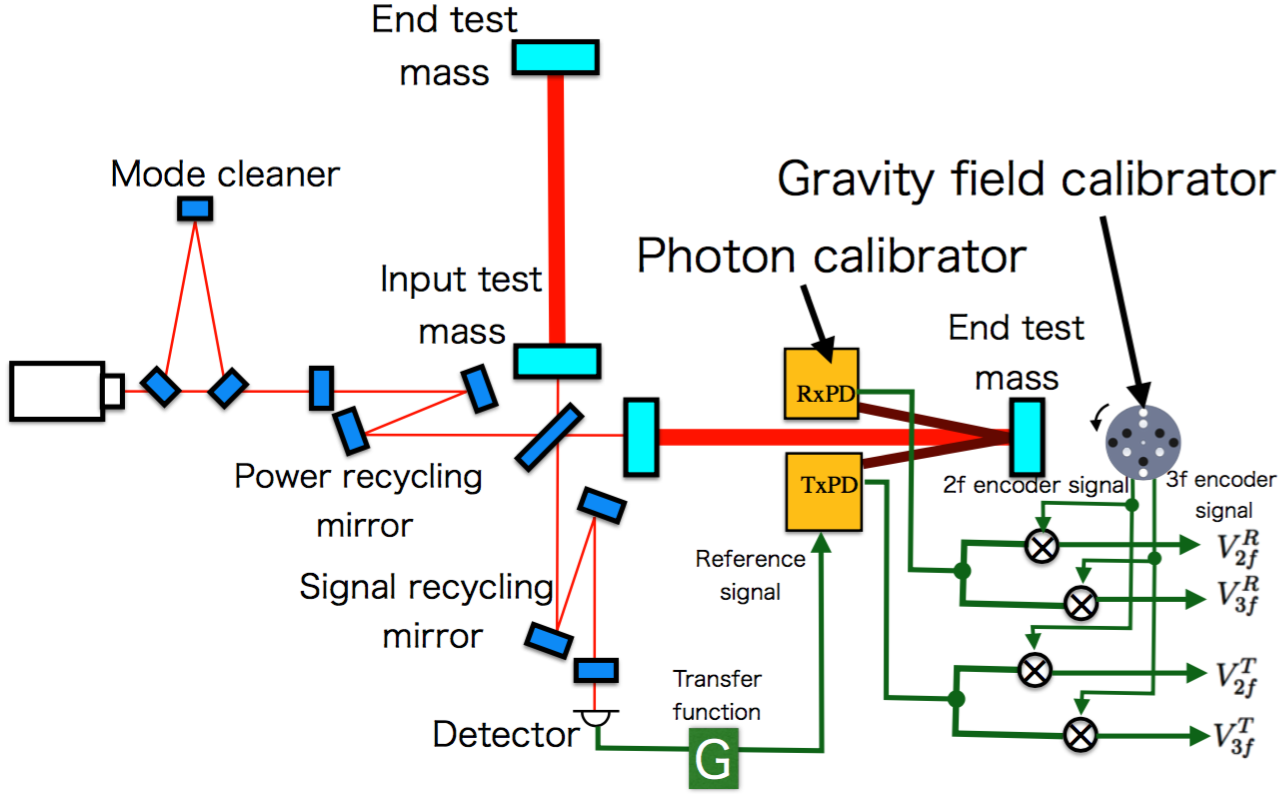
\includegraphics[width=12cm]{IFO.eps}
\caption{Test setup of the calibration of the laser power by rotating gravity field calibrator.}
\label{fig:IFO}
\end{center}
\end{figure}

\section{Estimation of uncertainty} \label{sec:EST}
In evaluating the accuracy of the estimated displacement, we discuss the systematic error by changing the operation frequency and distance. After that, we discuss the uncertainty of the displacement of the mirror. 
We estimate the uncertainty of the displacement by assuming KAGRA basic parameter as shown in Fig.~\ref{pcal}. The assumed parameters of the calibrators are listed in Table~\ref{sus}. We assumed these number in the following section.

\begin{table}
\begin{center}
\caption{\label{sus}The assumed parameters.}
\footnotesize
\begin{tabular}{cccc}
\hline
&&Value&Relative uncertainty \\
\hline
$G$& Gravity constant&$6.6742 \times 10^{-11}~\mathrm{[m^3kg^{-1}sec^{-2}]}$&0.015 \%\\
%$c$& speed of light&$2.99792458 \times 10^8$ [m/sec]& 0\%\\
$\cos{\theta}$& Incident angle&1.000& 0.07~\%\\
$M$& Mass of test mass&22.89~[kg] & 0.02~\%\\
$m_{\mathrm{q}}$&Mass of quadrupole&4.485~[kg] & 0.004~\%\\
$m_{\mathrm{h}}$&Mass of hexapole& 4.485~[kg] &0.004~\%\\
$r_{\mathrm{q}}$&Radius of quadrupole&0.200~[m] & 0.01~\%\\
$r_{\mathrm{h}}$&Radius of hexapole& 0.125~[m] & 0.02~\%\\
$1+\frac{I}{M}\vec{a}\cdot \vec{b}$& Geometrical factor & 1&0.3~\% \\
\hline
\end{tabular}\\
\end{center}
\end{table}

\subsection{Systematic error of the higher order term}
In order to achieve the precision less than 1 \%, we need to consider the operation position due to the higher order of Legendre polynomial. This is because that higher order also include the 2-f and 3-f components. The order of the Legendre polynomial is characterized by n as shown in Eq.(\ref{eq:EOM}). The effect of higher order factor is mitigated by the factor of $(r/d)^n$. Table~\ref{tab:N2} and \ref{tab:N3} shows the calculated displacement of the higher order term. To compare the higher order effect, we calculate the ratio between the FEM and calculation by changing the r/d is shown in Fig~\ref{fig:FEM}. We need to place the mirror at least 2~m away from the mirror to reduce the systematic error. In the following calculation, we assume the distance as 2~m. 

\begin{table}
\begin{center}
\caption{The calculated quadrupole($N=2$) displacement. $n$ is order of Legendre polynomial, where $\omega=n\omega_{\mathrm{rot}}$. \label{tab:N2}}
\footnotesize
\begin{tabular}{cccccccc}
\hline
modulation& n=1 & n=2& n=3 &n=4&n=5&n=6&n=7 \\
\hline
1f&0&0&0&0&0&0&0 \\
2f&0&$9 \frac{Gmr^2}{d^4\omega^2}$&0&$\frac{25}{4} \frac{Gmr^4}{d^6\omega^2}$&0&$\frac{735}{128} \frac{Gmr^6}{d^8\omega^2}$&0  \\
3f&0&0&0&0&0&0&0\\
4f&0&0&0&$\frac{175}{16} \frac{Gmr^4}{d^6\omega^2}$&0& $\frac{441}{64} \frac{Gmr^6}{d^8\omega^2}$&0 \\
5f&0&0&0&0&0&0&0 \\
6f&0&0&0&0&0&$\frac{1617}{128} \frac{Gmr^6}{d^8\omega^2}$&0  \\
\hline
\end{tabular}
\end{center}
\end{table}

\begin{table}
\begin{center}
\caption{The calculated hexapole($N=3$) displacement. $n$ is order of Legendre polynomial, where $\omega=n\omega_{\mathrm{rot}}$.  \label{tab:N3}}
\footnotesize
\begin{tabular}{cccccccc}
\hline
modulation& n=1 & n=2& n=3 &n=4&n=5&n=6&n=7 \\
\hline
1f&0&0&0&0&0&0&0 \\
2f&0&0&0&0&0&0&0  \\
3f&0&0&$15\frac{Gmr^3}{d^5\omega^2}$&0&$\frac{315}{32}\frac{Gmr^5}{d^7\omega^2}$&0& $\frac{189}{64} \frac{Gmr^7}{d^9 \omega^2}$\\
4f&0&0&0&0&0&0&0 \\
5f&0&0&0&0&0&0&0 \\
6f&0&0&0&0&0&$\frac{4851}{256} \frac{Gmr^6}{d^8\omega^2}$&0  \\
\hline
\end{tabular}
\end{center}
\end{table}

\begin{figure}
\begin{center}
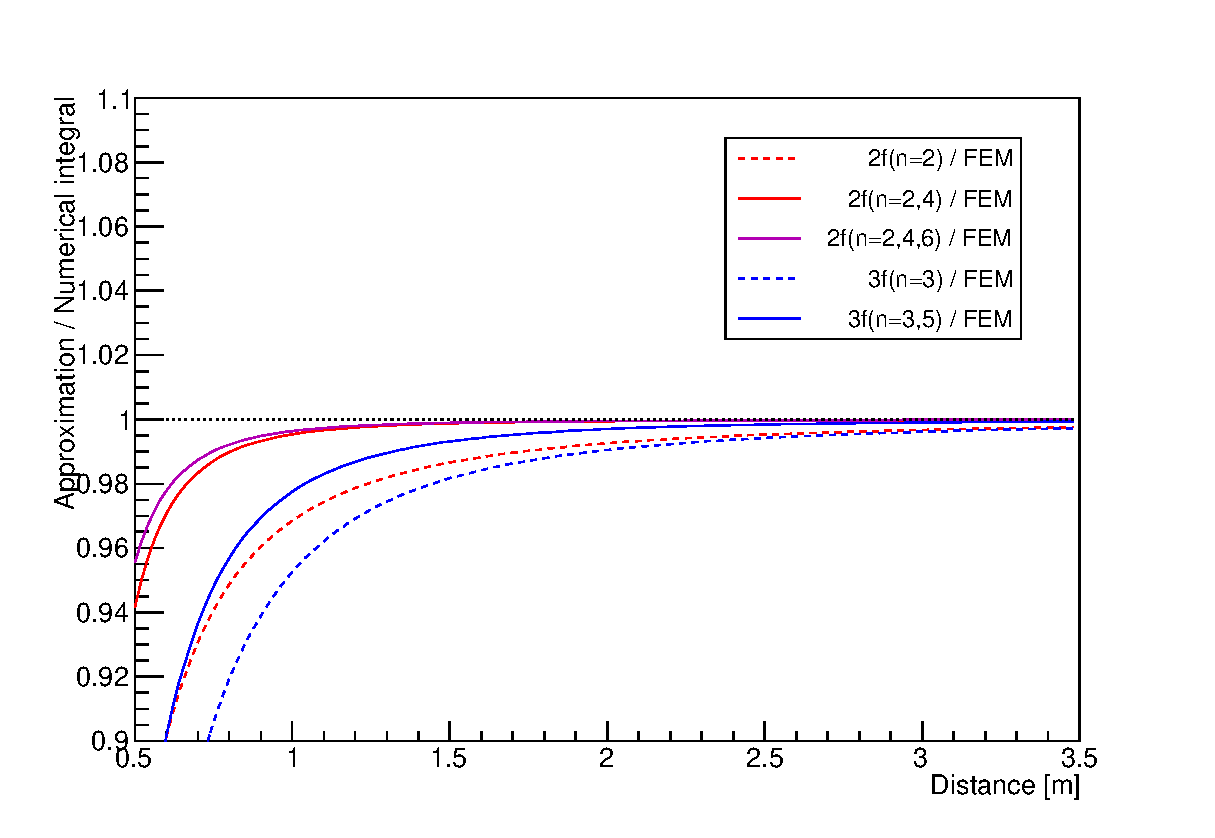
\includegraphics[width=12cm]{dvsx_ratio.eps}
\caption{The displacement ratio of the higher order effect by changing $r/d$. Dashed curves are included with the 1st order term. Solid curves are included with sum of 1st order and 2nd order. The analytical result is listed in Table~\ref{tab:N2} and~\ref{tab:N3}. To achieve the precision less than 1~\%, we need include the higher order terms.}
\label{fig:FEM}
\end{center}
\end{figure}


\subsection{Systematic error of the transfer function}
The gravity field calibrator can modulate the mirrors with gradient of gravity potential. However, its gravity gradient act the masses of suspension system as shown in Fig.~\ref{fig:cryo}. We simulated the transfer function between each mass and test mass.The transfer function is calculated by the suspension rigid-body simulation code, called SUMCON~\cite{`}. We estimated the total displacement including all the masses. Figure \ref{fig:ratio} shows the displacement ratio between the sensed motion and free mass motion as a function of frequency The structures of low frequency are corresponding to the resonant peak of the suspension system. We can neglect the intermediate mass effect and regard as free mass motion larger than 10~Hz. We assumed the rotation frequency as 16~Hz, which is corresponding to 32~Hz and 48~Hz at the operation frequency. of 2-f and 3-f components.  We used this assumption in the following section.
\begin{figure}
\begin{center}
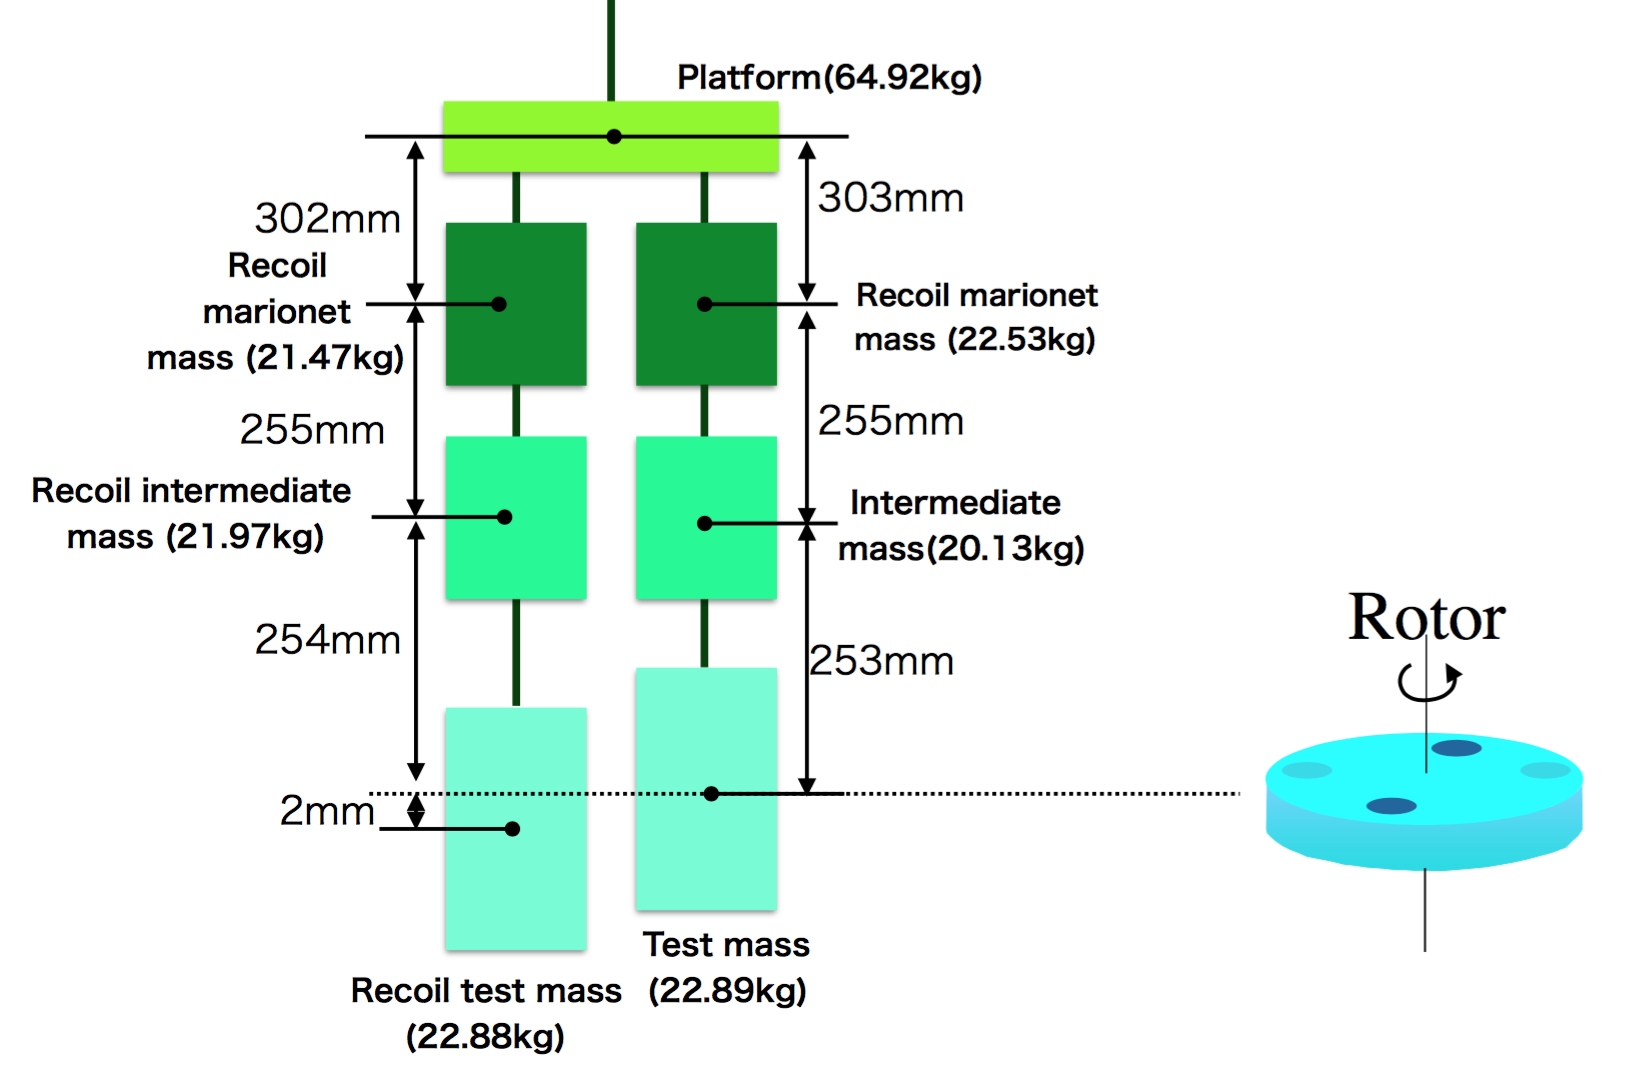
\includegraphics[width=12cm]{Cryo.eps}
\caption{Schematic view of the suspension system. The parameter of the hight and mass is the assumed value. }
\label{fig:cryo}
\end{center}
\end{figure}

\begin{figure}
\begin{center}
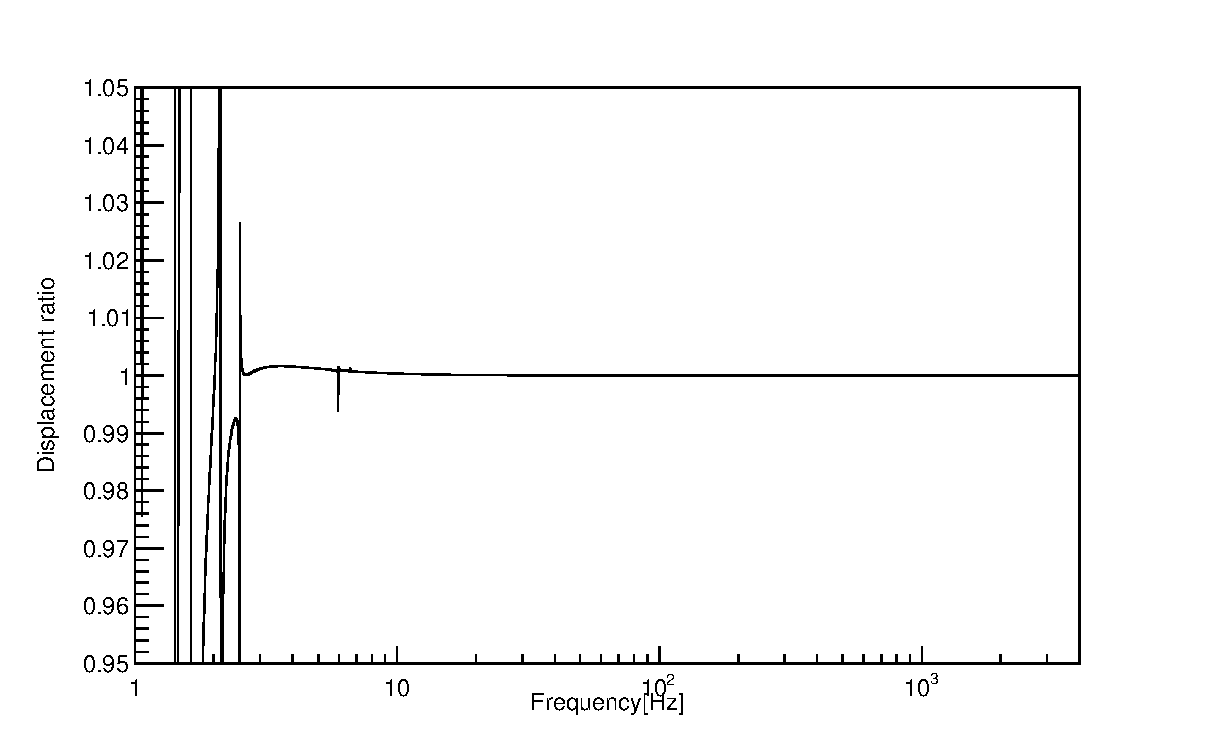
\includegraphics[width=12cm]{dx_Gcal_ratio.eps}
\caption{The displacement ratio of the transfer function of multi pendulum by changing modulation frequency, where relations of the modulation frequency, $f$, modulation angular frequency, $\omega$, and rotation angular frequency, $\omega_{\mathrm{rot}}$ are described as. $n\omega_{\mathrm{rot}}=\omega=2\pi f$. If we put the gravity field calibrator, it act the upper masses and it makes systematic error of the transfer function.}
\label{fig:ratio}
\end{center}
\end{figure}


\subsection{Uncertainty of displacement and  laser power}
In this section, we estimate the typical displacement based on the Table.~\ref{sus}. 
 The estimated displacements of 2-f and 3-f are described as
\begin{eqnarray}
x^{\mathrm{rms}}_{\mathrm{2f}}&=&1.178 \times 10^{-16}\mathrm{[m]} \times \left( \frac{G}{6.6742 \times 10^{-11} \mathrm{[m^3kg^{-1}sec^{-2}]}} \right) \times \left( \frac{m_{\mathrm{q}}}{4.485 \mathrm{[kg]}} \right) \times \left( \frac{r_{\mathrm{q}}}{0.200 \mathrm{[m]}} \right)^2 \nonumber \\
 &&\times \left( \frac{2\mathrm{[m]}}{d} \right)^4 \times \left( \frac{2\pi(2\times 16)\mathrm{[Hz]}}{\omega} \right)^2\\
x^{\mathrm{rms}}_{\mathrm{3f}}&=&2.130 \times 10^{-18}\mathrm{[m]} \times \left( \frac{G}{6.6742 \times 10^{-11} \mathrm{[m^3kg^{-1}sec^{-2}]}} \right) \times \left( \frac{m_{\mathrm{h}}}{4.485 \mathrm{[kg]}} \right) \times \left( \frac{r_{\mathrm{h}}}{0.125 \mathrm{[m]}} \right)^3 \nonumber \\
 &&\times \left( \frac{2\mathrm{[m]}}{d} \right)^5 \times \left( \frac{2\pi(3\times 16)\mathrm{[Hz]}}{\omega} \right)^2.
\end{eqnarray}
We defined the signal-to-noise ratio (SNR) with the ratio of RMS displacement to the design noise spectrum density of IFO of KAGRA at 32~Hz for 2-f and 48~Hz for 3-f.
By using this result, we estimate the signal to noise ratio of the peaks.
\begin{eqnarray}
SNR_{\mathrm{2f}}=392 \times \left(\frac{3.0 \times 10^{-19} \mathrm{m/\sqrt{Hz}}}{n_{\mathrm{32Hz}}} \right) \times \left(\frac{T}{1 [\mathrm{sec}]} \right)^{1/2} \times \left(\frac{x_{\mathrm{2f}}^{\mathrm{rms}}}{1.178 \times 10^{-16}\mathrm{[m]} }  \right),   \\
SNR_{\mathrm{3f}}=73 \times \left(\frac{2.9 \times 10^{-20} \mathrm{m/\sqrt{Hz}}}{n_{\mathrm{48Hz}}} \right) \times \left(\frac{T}{1 [\mathrm{sec}]} \right)^{1/2} \times \left(\frac{x_{\mathrm{2f}}^{\mathrm{rms}}}{2.130 \times 10^{-18}\mathrm{[m] }} \right)   \\
\end{eqnarray}
where $T$ is integration time. When we integrate the signal larger than 10 min, we can measure the $V^{\mathrm{R}}_{2f}$ and $V^{\mathrm{R}}_{3f}$ with enough of SNR.
We can apply this system for the measurement of the absolute laser power. The estimated powers are
\begin{eqnarray}
P_{\mathrm{2f}}&=&0.09288 ~\mathrm{[W]}\times \left( \frac{G}{6.6742 \times 10^{-11} \mathrm{[m^3kg^{-1}sec^{-2}]}} \right) \nonumber \\
&& \times \left( \frac{m_{\mathrm{q}}}{4.485 \mathrm{[kg]}} \right) \times \left( \frac{r_{\mathrm{q}}}{0.200 \mathrm{[m]}} \right)^2 \times \left( \frac{2\mathrm{[m]}}{d} \right)^4 \times \left( \frac{1}{\cos{\theta}} \right) \times \left( \frac{1}{1+\frac{M}{I}\vec{a}\cdot \vec{b}} \right)^2\\
P_{\mathrm{3f}}&=&0.003779~\mathrm{[W]} \times \left( \frac{G}{6.6742 \times 10^{-11} \mathrm{[m^3kg^{-1}sec^{-2}]}} \right) \nonumber \\
&& \times \left( \frac{m_{\mathrm{h}}}{4.485 \mathrm{[kg]}} \right) \times \left( \frac{r_{\mathrm{h}}}{0.125 \mathrm{[m]}} \right)^3 \times \left( \frac{2\mathrm{[m]}}{d} \right)^5 \times \left( \frac{1}{\cos{\theta}} \right) \times \left( \frac{1}{1+\frac{M}{I}\vec{a}\cdot \vec{b}} \right)^2.
\end{eqnarray}
The estimated $V^{\mathrm{T}}_{\mathrm{2f}}/V^{T}_{\mathrm{3f}}$ by changing distance are shown in Fig.~\ref{fig:dvsVV}.

\begin{figure}
\begin{center}
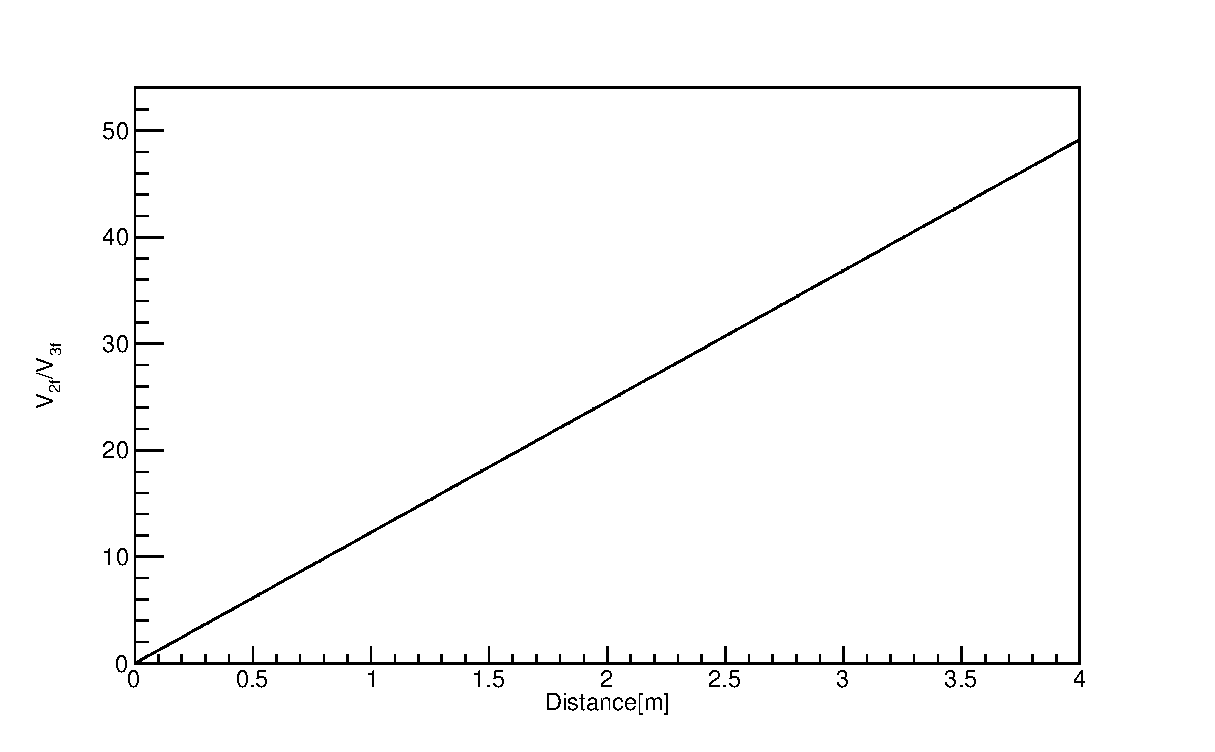
\includegraphics[width=12cm]{dvsVV.eps}
\caption{The response of $V_{\mathrm{2f}}/V_{\mathrm{3f}}$ by changing distance between test mass and gravity field calibrator.}
\label{fig:dvsVV}
\end{center}
\end{figure}
We can also estimate the laser power by using the following equations:
\begin{eqnarray}
\left( \frac{\delta P_{\mathrm{2f}}}{P_{\mathrm{2f}}} \right)^2 &\sim& \left( \frac{\delta G}{G} \right)^2 + \left( \frac{\delta M}{M} \right)^2+25\left( \frac{\delta m_{\mathrm{q}}}{m_{\mathrm{q}}} \right)^2+16\left( \frac{\delta m_{\mathrm{h}}}{m_{\mathrm{h}}} \right)^2 +100\left( \frac{\delta r_{\mathrm{q}}}{r_{\mathrm{q}}} \right)^2+144\left( \frac{\delta r_{\mathrm{h}}}{r_{\mathrm{h}}} \right)^2 \nonumber \\
&+&16\left( \frac{\delta V^{\mathrm{R}}_{{\mathrm{2f}}}}{V^{\mathrm{R}}_{{\mathrm{2f}}}} \right)^2+16\left( \frac{\delta V^{\mathrm{R}}_{{\mathrm{2f}}}}{V^{\mathrm{R}}_{{\mathrm{2f}}}} \right)^2+\left( \frac{\delta (\cos{\theta})}{\cos{\theta}} \right)^2+ \left( \frac{\delta\left( 1+\frac{M}{I}\vec{a}\cdot \vec{b} \right)}{\left( 1+\frac{M}{I}\vec{a}\cdot \vec{b} \right)} \right)^2 \\
\left( \frac{\delta P_{\mathrm{3f}}}{P_{\mathrm{3f}}} \right)^2 &\sim& \left( \frac{\delta G}{G} \right)^2 + \left( \frac{\delta M}{M} \right)^2+25\left( \frac{\delta m_{\mathrm{q}}}{m_{\mathrm{q}}} \right)^2+16\left( \frac{\delta m_{\mathrm{h}}}{m_{\mathrm{h}}} \right)^2 +100\left( \frac{\delta r_{\mathrm{q}}}{r_{\mathrm{q}}} \right)^2+144\left( \frac{\delta r_{\mathrm{h}}}{r_{\mathrm{h}}} \right)^2 \nonumber \\
&+&16\left( \frac{\delta V^{\mathrm{R}}_{{\mathrm{2f}}}}{V^{\mathrm{R}}_{{\mathrm{2f}}}} \right)^2+16\left( \frac{\delta V^{\mathrm{R}}_{{\mathrm{2f}}}}{V^{\mathrm{R}}_{{\mathrm{2f}}}} \right)^2+\left( \frac{\delta (\cos{\theta})}{\cos{\theta}} \right)^2+ \left( \frac{\delta\left( 1+\frac{M}{I}\vec{a}\cdot \vec{b} \right)}{\left( 1+\frac{M}{I}\vec{a}\cdot \vec{b} \right)} \right)^2 
\end{eqnarray}
The uncertainty of the quadrupole and hexapole masses are limited by the accuracy of electronic balance. In this case, we use the weight made of Tungsten. The density of Tungsten is $19.25~\mathrm{g/cm^3}$. The diameter and thickness of mass are 0.06m and 0.08~m, respectively. Therefore, the mass of the rotor mass is 4.485~kg. To measure this mass, we assumed that we use an electronic balance whose catalog number and accuracy are CG-6000 and 0.2~g, respectively. Therefore, the relative uncertainty of the mass of rotor mass is 0.04~\%.

 To make the rotor disk, we use the NC milling machine. The typical accuracy is less than 0.02 mm. For the measuring of the shape, we employ the three-dimension coordinate measuring machine (CMM)~\cite{Inoue:2016kyq}. The precision of CMM is $2~\mathrm{\mu m}$. We can measure the shape of the rotor and masses with enough of uncertainty using CMM. 

The estimated relative uncertainties of the powers are 0.4\%. One of the largest uncertainty is the geometrical factor of the Pcal laser. The geometrical factor uncertainty is assumed 0.3 \%, which is same number of LIGO. 

 Finally, the estimated relative uncertainty of  displacement is written as
\begin{eqnarray}
\left( \frac{\delta x}{x} \right)^2 &\sim& \left( \frac{\delta G}{G} \right)^2 +\left( \frac{\delta V_{in}}{V_{in}} \right)^2+\left( \frac{\delta M}{M} \right)^2+\left( \frac{\delta s(\omega)}{s(\omega)} \right)^2+ 25\left( \frac{\delta m_{\mathrm{q}}}{m_{\mathrm{q}}} \right)^2 +16\left( \frac{\delta m_{\mathrm{h}}}{m_{\mathrm{h}}} \right)^2 \nonumber \\
&+&25\left( \frac{\delta V^{\mathrm{R}}_{{\mathrm{2f}}}}{V^{\mathrm{R}}_{{\mathrm{2f}}}} \right)^2+16\left( \frac{\delta V^{\mathrm{R}}_{{\mathrm{2f}}}}{V^{\mathrm{R}}_{{\mathrm{2f}}}} \right)^2+ 100\left( \frac{\delta r_{\mathrm{q}}}{r_{\mathrm{q}}} \right)^2 +144\left( \frac{\delta r_{\mathrm{h}}}{r_{\mathrm{h}}} \right)^2. \label{deltax}
\end{eqnarray}
The contribution of the radius uncertainty is amplified by the O(100) factor. To reduce the noise of displacement, we need to reduce the uncertainty of the shape of the rotor and masses.
The uncertainty of the $V^{\mathrm{R}}_{\mathrm{2f}}$,$V^{\mathrm{R}}_{\mathrm{3f}}$, $V^{\mathrm{R}}_{0}$ are much less than other contributions.We can reduce the uncertainty of these values with long time integration time due to the statistics. Each the uncertainty is listed in Table.~\ref{sus}. The estimated  total uncertainty of the displacement is 0.3~\%.

% Added by SH 180414
\begin{table}
\begin{center}
\caption{Comparison of systematic error contributions between eq.~\ref{deltax} and Monte Carlo simulation. \label{tab:MC}}
\begin{tabular}{ccccc}
\hline
&&Relative uncertainty&Contribution(eq.~\ref{deltax})&Contribution(MC simulation)\\
\hline
$G$& Gravity constant&0.015 \%&0.015 \%&0.015 \%\\
$M$& Mass of test mass& 0.02~\%& 0.02~\%& 0.02~\%\\
$m_{\mathrm{q}}$&Mass of poles& 0.004~\% & 0.025~\% & 0.022~\%\\
$r_{\mathrm{q}}$&Radius of poles& 0.01/0.02~\%& 0.26~\%& 0.028~\%\\
$V^{\mathrm{R}}$&Demodulated signal& 0.001~\%& 0.006~\%& 0.006~\%\\
\hline\hline
$x$&displacement&& 0.26~\%& 0.048~\%\\
\hline
\end{tabular}\\
\end{center}
\end{table}
% Added by SH 180414

\section{Conclusion}
Photon calibrator is one of the powerful calibrators in advanced LIGO, advanced Virgo and KAGRA. It can calibrate the response of IFO and its uncertainty is essential for estimation of gravitational wave source. In particular, the distance of the source is strongly depend on the absolute laser power of the photon calibrator. In previous study, the Gold standard, which response is calibrated by the laser power standard of NIST, is used for the absolute laser power calibration of the photon calibrator. However, current limit of the absolute laser power between each country is about 3.5~\%. It is directly propagate to the uncertainty of absolute displacement of gravitational wave detector.

To solve the problem, we proposed the combination method of photon calibrator and gravity field calibrator. Gravity field calibrator can modulate the mirror using gravity gradient. By canceling the displacement of the test mass using the photon calibrator, we can calibrate the absolute laser power and displacement of the photon calibrator with accuracy of 0.4~\% and 0.3~\%.

This method has an advantage of a direct comparison of the amplitude of injected power and gravity field. In previous study, we need to consider the uncertainty of the optical efficiency through the window and mirrors. This is because we put the working standard at the outside of the chamber. However, the method of gravity field can compare the displacement directly. By using this method, we can calibrate the uncertainty of optical efficiency and absolute power of the laser. When we compare the laser power between each institute, we need to bring the working standard. However, we can try the absolute calibration using this method. As we mention about a few percent of the absolute uncertainty of laser in each country. The estimated uncertainty of the power of this method is 0.4\%. It imply that we can make a new power standard using interferometer.
%%%%%%%%%%%%%%%%%%%%%%%%%%%%%%%%%%%%%%%%%%%%%%%%%%%%%%%%%%%%%
\acknowledgments     %>>>> equivalent to \section*{ACKNOWLEDGMENTS}       
 
We thank Rechard Savage, Darkhan Tuyrnbayev for discussion of the photon calibrator. We would like to express our gratitude to Prof.Takaaki Kajita and Prof.Henry Wong. We would like to thank the KEK Cryogenics Science Center for the support. YI was supported by Academia Sinica under Grants No. CDA-105-M06 in Taiwan. This work was supported by JSPS KAKENHI Grant Numbers 17H106133 and XXXXXX. This work was supported by MEXT, JSPS Leading-edge Research Infrastructure Program, JSPS Grant-in-Aid for Specially Promoted
Research 26000005, MEXT Grant-in-Aid for Scientific Research on
Innovative Areas 24103005, JSPS Core-to-Core Program, A. Advanced
Research Networks, and the joint research program of the Institute for
Cosmic Ray Research, University of Tokyo.

%%%%%%%%%%%%%%%%%%%%%%%%%%%%%%%%%%%%%%%%%%%%%%%%%%%%%%%%%%%%%
%%%%% References %%%%%

\bibliography{report}   %>>>> bibliography data in report.bib
\bibliographystyle{spiebib}   %>>>> makes bibtex use spiebib.bst

\end{document} 
